% Solution to the Lecture 3 mini case (Aula/Lecture03.pdf, PDF pages 77-78 = deck slides 41-42): work or shirk?
% Compile: pdflatex mini-case-lecture-03.tex (twice). Check: pdffonts (all Type 1, uni = yes).
% Every number is asserted by mini-case-lecture-03-check.py in this folder.
\documentclass[11pt,a4paper]{article}
\usepackage[utf8]{inputenc}
\usepackage[T1]{fontenc}
\usepackage{lmodern}   % Type 1 vector fonts (replaces PK bitmaps)
\usepackage{cmap}      % ToUnicode CMap -> copyable text and accents
\usepackage[english]{babel}
\usepackage{amsmath,amssymb,amsthm,mathtools}
\usepackage[a4paper,margin=2.4cm]{geometry}
\usepackage{microtype}
\usepackage{booktabs,array,multirow}
\usepackage{enumitem}
\usepackage{xcolor}
\usepackage{tikz}
\usetikzlibrary{arrows.meta,positioning,calc}
\usepackage[most]{tcolorbox}
\usepackage{fancyhdr}
\usepackage[hidelinks]{hyperref}

\setlist{topsep=3pt,itemsep=2pt}
\setlength{\parindent}{0pt}
\setlength{\parskip}{5pt}
\renewcommand{\arraystretch}{1.2}
\allowdisplaybreaks

\pagestyle{fancy}\fancyhf{}
\lhead{\footnotesize Economics of Organizations and Incentives --- MPE Insper}
\rhead{\footnotesize Lecture 3 mini case: solution}
\cfoot{\footnotesize\thepage}
\renewcommand{\headrulewidth}{0.3pt}
\setlength{\headheight}{14pt}

\definecolor{ans}{RGB}{20,110,70}
\definecolor{src}{RGB}{30,80,150}
\definecolor{emp}{RGB}{190,60,40}
\definecolor{mgr}{RGB}{30,80,150}
\newcommand{\answer}[1]{\begin{tcolorbox}[colback=ans!5,colframe=ans,boxrule=0.6pt,
  left=5pt,right=5pt,top=3pt,bottom=3pt]\textbf{Answer.} #1\end{tcolorbox}}
\newenvironment{notacao}{\par\smallskip\noindent\textbf{Notation.}\begin{itemize}[leftmargin=1.4em,topsep=1pt,itemsep=0pt]\small}{\end{itemize}}
\newcommand{\supp}{\operatorname{supp}}

\title{\textbf{Mini Case, Lecture 3: Work or Shirk?}\\[4pt]
  \large Solution --- Economics of Organizations and Incentives (MPE Insper)}
\date{November 2026}

\begin{document}
\maketitle
\thispagestyle{empty}

\section*{The case}

\textbf{Source.} Lecture 3 slides (\texttt{Aula/Lecture03.pdf}), PDF pages 77--78 (deck slides
41--42), ``Mini case: work or shirk?'' and ``Mini case: questions''; motivation on PDF pages 74--76
(deck slide 40): in September 2025 Itaú dismissed employees after finding mismatches between their
clock-in records and the activity monitored on their computers while working from home (the bank
workers' union estimated about 1,000 dismissals; source on the slide: g1, 2025). Reproduced verbatim.

\begin{tcolorbox}[colback=src!4,colframe=src,boxrule=0.5pt]
A remote employee chooses to \textbf{work} ($W$) or \textbf{shirk} ($S$); at the same time, the
manager chooses to \textbf{monitor} ($M$) or \textbf{not} ($N$). A shirker who is caught loses the
wage.

\begin{center}
\begin{tabular}{cc|c|c|}
 & \multicolumn{3}{c}{Manager}\\
 & \multicolumn{1}{c}{} & \multicolumn{1}{c}{$M$} & \multicolumn{1}{c}{$N$}\\ \cline{3-4}
\multirow{2}{*}{Employee} & $W$ & $w-g,\ v-w-h$ & $w-g,\ v-w$ \\ \cline{3-4}
 & $S$ & $0,\ -h$ & $w,\ -w$ \\ \cline{3-4}
\end{tabular}
\qquad
\begin{tabular}{@{}l@{\ \ }l@{}}
\multicolumn{2}{@{}l}{\textbf{Parameters}}\\
$w = 10$ & wage\\
$g = 2$ & cost of effort\\
$v = 20$ & value of output\\
$h = 1$ & cost of monitoring
\end{tabular}
\end{center}

\textbf{Mini case: questions (in pairs, hand in today)}
\begin{enumerate}[label=(\alph*)]
  \item Show that the game has no Nash equilibrium in pure strategies.
  \item Find the mixed-strategy Nash equilibrium: the probability of shirking and the probability
        of monitoring.
  \item The firm buys cheaper monitoring software, and $h$ falls from 1 to 0.5. What happens to
        shirking? And to monitoring? Explain the intuition.
  \item The firm raises the wage to $w = 20$. What happens to shirking and to monitoring?
  \item Write the equilibrium probabilities as functions of $w$, $g$ and $h$. Which policy would you
        recommend to the firm, and which assumptions of the model would you question in the Itaú
        case?
\end{enumerate}
\end{tcolorbox}

\textbf{Method.} Mixed strategies and expected payoffs (deck slides 8--9), mixed-strategy Nash
equilibrium and the principle of indifference (slides 10--12), the battle of the sexes worked by
best-response diagrams (slides 13--16), interpretations of mixing (slide 17); Tadelis (2013)
\S6.1--6.2, pp.~101--114 (Def.~6.6, p.~107; Prop.~6.1, p.~108; the ``indifference logic'' and
``bosses monitoring employees'', p.~111). The commitment variant in (e) uses the Lecture 3 dynamic
material: sequential rationality and backward induction (slides 29--30), subgame perfection (slide
34) and Stackelberg (slide 37); Tadelis \S8.3.2 (pp.~160--163) and \S8.3.4 (pp.~166--169). The
closest book exercise is Tadelis 6.4 ``Monitoring'' (pp.~123--124). Every number below is asserted
by \texttt{Resolucao/mini-case-lecture-03-check.py}.

\begin{notacao}
  \item $I = \{E, M\!g\}$: the employee (rows) and the manager (columns); $S_E = \{W, S\}$,
        $S_{M\!g} = \{M, N\}$.
  \item $u_E$, $u_{M\!g}$: payoffs, as in the matrix; the manager's payoff is the firm's profit.
  \item $p = \sigma_E(S) = \Pr(\text{shirk})$, $q = \sigma_{M\!g}(M) = \Pr(\text{monitor})$, both in
        $[0, 1]$; equilibrium values $p^*$, $q^*$.
  \item $u_E(W, q)$: the employee's expected payoff from $W$ when the manager monitors with probability
        $q$ (slide 9's $u_i(s_i, \sigma_{-i})$); likewise $u_E(S, q)$, $u_{M\!g}(M, p)$, $u_{M\!g}(N, p)$.
  \item $\pi(w, h) := u_{M\!g}^*$: the firm's equilibrium payoff as a function of the parameters.
  \item $\delta \in (0, 1]$: probability that monitoring detects a shirker (used only in (e); the case
        has $\delta = 1$).
\end{notacao}

%-------------------------------------------------------------------------------------------
\section*{Setup}

A simultaneous-move game of complete information, $G = (I, \{S_i\}, \{u_i\})$. Reading the cells:
the employee is paid $w$ unless caught shirking, and pays the effort cost $g$ only when working; the
firm gets output $v$ only when the employee works, pays $w$ unless it catches a shirker, and pays $h$
whenever it monitors. Substituting $w = 10$, $g = 2$, $v = 20$, $h = 1$
($w - g = 8$, $v - w - h = 9$, $v - w = 10$):
\begin{center}
\begin{tabular}{c|cc}
$E \backslash M\!g$ & $M$ & $N$ \\ \midrule
$W$ & $8,\ 9$ & $8,\ 10$ \\
$S$ & $0,\ -1$ & $10,\ -10$
\end{tabular}
\end{center}
The game is the \emph{inspection game}: the employee wants to shirk exactly when he is not watched,
and the manager wants to watch exactly when the employee shirks, so each wants to outguess the other
(Tadelis p.~111 lists ``bosses monitoring employees'' among such games).

%-------------------------------------------------------------------------------------------
\section*{(a) No Nash equilibrium in pure strategies}

A pure profile is a Nash equilibrium if neither player gains by switching alone. Check each cell
(the deviating player's payoffs before $\to$ after):
\begin{itemize}
  \item $(W, M)$: the manager switches to $N$: $9 \to 10$, gain $h = 1$ (monitoring a worker costs $h$
        and catches no one).
  \item $(W, N)$: the employee switches to $S$: $8 \to 10$, gain $g = 2$ (unwatched, he saves the
        effort cost).
  \item $(S, N)$: the manager switches to $M$: $-10 \to -1$, gain $w - h = 9$ (catching the shirker
        saves the wage at cost $h$).
  \item $(S, M)$: the employee switches to $W$: $0 \to 8$, gain $w - g = 8$ (working keeps the wage).
\end{itemize}
Every cell has a profitable unilateral deviation, so no cell is a Nash equilibrium. The deviations
chain into a cycle (arrows: who deviates; underlined: best-response payoffs):

\begin{center}
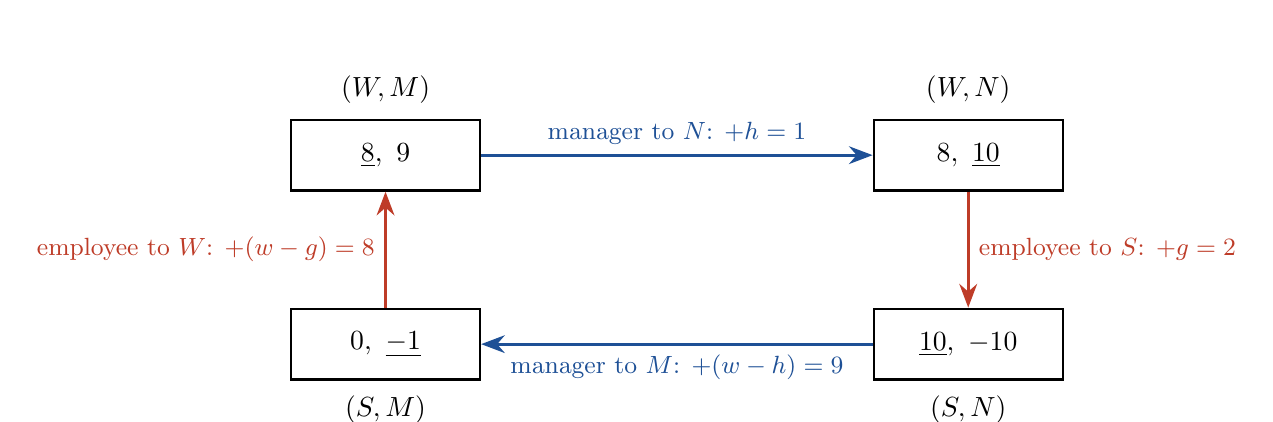
\begin{tikzpicture}[cell/.style={draw,thick,minimum width=2.4cm,minimum height=0.9cm},
  dev/.style={-{Stealth[length=3mm]},line width=1.1pt}]
  \node[cell] (WM) at (0,0) {$\underline{8},\ 9$};
  \node[cell] (WN) at (7.4,0) {$8,\ \underline{10}$};
  \node[cell] (SM) at (0,-2.4) {$0,\ \underline{-1}$};
  \node[cell] (SN) at (7.4,-2.4) {$\underline{10},\ -10$};
  \node[above=2pt of WM] {$(W, M)$}; \node[above=2pt of WN] {$(W, N)$};
  \node[below=2pt of SM] {$(S, M)$}; \node[below=2pt of SN] {$(S, N)$};
  \draw[dev,mgr] (WM.east) -- node[above,font=\small] {manager to $N$: $+h = 1$} (WN.west);
  \draw[dev,emp] (WN.south) -- node[right,font=\small] {employee to $S$: $+g = 2$} (SN.north);
  \draw[dev,mgr] (SN.west) -- node[below,font=\small] {manager to $M$: $+(w - h) = 9$} (SM.east);
  \draw[dev,emp] (SM.north) -- node[left,font=\small] {employee to $W$: $+(w - g) = 8$} (WM.south);
\end{tikzpicture}
\end{center}

The employee's best response is $W$ against $M$ ($8 > 0$) and $S$ against $N$ ($10 > 8$); the
manager's is $N$ against $W$ ($10 > 9$) and $M$ against $S$ ($-1 > -10$). No cell has both payoffs
underlined.

\textbf{In general.} The four gains around the cycle are $h$, $g$, $w - h$ and $w - g$. All are
positive, so there is no pure equilibrium, whenever
\[
  0 < g < w \qquad\text{and}\qquad 0 < h < w,
\]
that is: effort is costly but worth less than the wage, and monitoring is costly but cheaper than
the wage it saves. With $g > w$ the employee would always shirk; with $h > w$ the manager would never
monitor.

\answer{Each cell has a profitable deviation: $(W,M) \to (W,N)$ (manager saves $h = 1$),
$(W,N) \to (S,N)$ (employee saves $g = 2$), $(S,N) \to (S,M)$ (manager gains $w - h = 9$),
$(S,M) \to (W,M)$ (employee gains $w - g = 8$). The best responses cycle, so there is no pure-strategy
Nash equilibrium; this holds whenever $0 < g < w$ and $0 < h < w$.}

%-------------------------------------------------------------------------------------------
\section*{(b) The mixed-strategy Nash equilibrium}

\textbf{Step 1: both players must mix.} If the manager played a pure strategy, the employee's best
response would be unique and pure ($W$ against $M$, $S$ against $N$), and the pair would be a pure
equilibrium, which (a) rules out. The same holds if the employee played a pure strategy. So in any
equilibrium $p, q \in (0, 1)$, both supports are full, and by the principle of indifference (slide 10,
condition 1; Tadelis Prop.~6.1, p.~108) \emph{each player must be indifferent between his two
actions}. Condition 2 (no better strategy outside the support) is then empty.

\textbf{Step 2: the employee's indifference pins $q$.} Against a manager who monitors with
probability $q$ (slide 9, $u_i(s_i, \sigma_{-i})$):
\begin{align}
  u_E(W, q) &= q\,(w - g) + (1 - q)(w - g) = w - g = 8, \label{eq:EW}\\
  u_E(S, q) &= q \cdot 0 + (1 - q)\, w = 10\,(1 - q) = 10 - 10q. \label{eq:ES}
\end{align}
Working pays $8$ whatever the manager does; shirking pays the wage only if not monitored. Setting
\eqref{eq:EW} equal to \eqref{eq:ES}:
\begin{align*}
  8 &= 10 - 10q\\
  10q &= 2\\
  q^* &= 0.2.
\end{align*}
In symbols, $u_E(S, q) - u_E(W, q) = g - q w$: shirking saves the effort cost $g$ and loses the wage
$w$ with probability $q$; it is zero at $q^* = g/w$.

\textbf{Step 3: the manager's indifference pins $p$.} Against an employee who shirks with
probability $p$:
\begin{align}
  u_{M\!g}(M, p) &= (1 - p)(v - w - h) + p\,(-h) = (1 - p)\cdot 9 - p = 9 - 10p, \label{eq:MM}\\
  u_{M\!g}(N, p) &= (1 - p)(v - w) + p\,(-w) = (1 - p)\cdot 10 - 10p = 10 - 20p. \label{eq:MN}
\end{align}
Setting \eqref{eq:MM} equal to \eqref{eq:MN}:
\begin{align*}
  9 - 10p &= 10 - 20p\\
  10p &= 1\\
  p^* &= 0.1.
\end{align*}
In symbols, $u_{M\!g}(M, p) - u_{M\!g}(N, p) = p w - h$: monitoring recovers the wage of a shirker
(probability $p$) at cost $h$; output $v$ cancels because monitoring does not change whether the work
gets done. It is zero at $p^* = h/w$.

\textbf{Step 4: best responses.} From \eqref{eq:EW}--\eqref{eq:MN}:
\[
  BR_E(q) = \begin{cases} S\ (p = 1) & q < 0.2,\\ \text{any } p \in [0,1] & q = 0.2,\\
  W\ (p = 0) & q > 0.2, \end{cases}
  \qquad
  BR_{M\!g}(p) = \begin{cases} N\ (q = 0) & p < 0.1,\\ \text{any } q \in [0,1] & p = 0.1,\\
  M\ (q = 1) & p > 0.1. \end{cases}
\]
The two correspondences cross once, at $(p^*, q^*) = (0.1, 0.2)$, so this is the unique Nash
equilibrium (Figure~\ref{fig:br}).

\begin{figure}[ht]
\centering
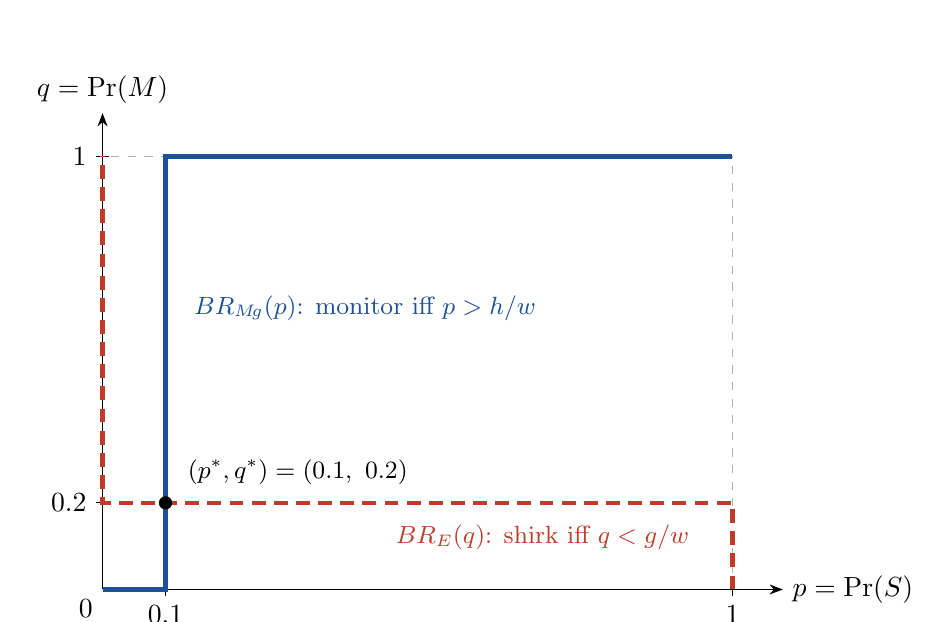
\begin{tikzpicture}[x=8cm,y=5.5cm,>=Stealth]
  \draw[->] (0,0) -- (1.08,0) node[right] {$p = \Pr(S)$};
  \draw[->] (0,0) -- (0,1.1) node[above] {$q = \Pr(M)$};
  \foreach \x/\l in {0.1/0.1, 1/1} \draw (\x,0.015) -- (\x,-0.015) node[below] {$\l$};
  \foreach \y/\l in {0.2/0.2, 1/1} \draw (0.01,\y) -- (-0.01,\y) node[left] {$\l$};
  \node[below left] at (0,0) {$0$};
  \draw[dashed,gray!60] (1,0) -- (1,1) -- (0,1);
  % manager: q as a function of p
  \draw[mgr,line width=1.6pt] (0,0) -- (0.1,0) -- (0.1,1) -- (1,1);
  % employee: p as a function of q
  \draw[emp,line width=1.6pt,dash pattern=on 5pt off 3pt] (1,0) -- (1,0.2) -- (0,0.2) -- (0,1);
  \fill (0.1,0.2) circle (2.4pt);
  \node[anchor=south west,font=\small] at (0.12,0.22) {$(p^*, q^*) = (0.1,\ 0.2)$};
  \node[mgr,font=\small,anchor=west] at (0.13,0.65) {$BR_{M\!g}(p)$: monitor iff $p > h/w$};
  \node[emp,font=\small,anchor=west] at (0.45,0.12) {$BR_E(q)$: shirk iff $q < g/w$};
\end{tikzpicture}
\caption{Best responses in $(p, q)$: manager solid, employee dashed. Each kink sits at the value
that makes the \emph{other} player indifferent. The arrows of (a) circle the square's corners; the
only mutual best response is interior.}
\label{fig:br}
\end{figure}

\textbf{Step 5: equilibrium payoffs.} Each player gets the payoff of either action in his support:
\begin{align*}
  u_E^* &= u_E(W, q^*) = 8 \quad\big(= u_E(S, q^*) = 10\,(1 - 0.2) = 8\big),\\
  u_{M\!g}^* &= u_{M\!g}(M, p^*) = 9 - 10(0.1) = 8 \quad\big(= u_{M\!g}(N, p^*) = 10 - 20(0.1) = 8\big).
\end{align*}
Check with the full formula $u_i(\sigma) = \sum_s \sigma_E(s_E)\,\sigma_{M\!g}(s_{M\!g})\,u_i(s)$
(slide 9). The outcome probabilities are
\begin{center}
\begin{tabular}{c|cc}
 & $M$ ($q^* = 0.2$) & $N$ ($0.8$) \\ \midrule
$W$ ($1 - p^* = 0.9$) & $0.18$ & $0.72$ \\
$S$ ($p^* = 0.1$) & $0.02$ & $0.08$
\end{tabular}
\end{center}
and the manager's expected payoff is $0.18(9) + 0.72(10) + 0.02(-1) + 0.08(-10) = 8$; the
employee's is $0.18(8) + 0.72(8) + 0.02(0) + 0.08(10) = 8$.

\textbf{Reading.} Under the population interpretation of slide 17, one employee in ten shirks, one
in five is monitored, and $2\%$ of the workforce is caught (the $(S, M)$ cell: the dismissals of the
Itaú story); another $8\%$ shirks undetected. Shirking and dismissals are an equilibrium outcome, not
a failure of the policy.

\answer{The unique Nash equilibrium is in mixed strategies: the employee shirks with probability
$p^* = h/w = 0.1$ and the manager monitors with probability $q^* = g/w = 0.2$. Payoffs: employee
$w - g = 8$, manager $(1 - p^*)(v - w) - h = 8$.}

%-------------------------------------------------------------------------------------------
\section*{(c) Cheaper monitoring: $h$ falls from 1 to 0.5}

\textbf{Employee.} $h$ does not appear in \eqref{eq:EW} or \eqref{eq:ES}, so
$u_E(W, q) = 8$ and $u_E(S, q) = 10 - 10q$ as before: $q^* = 0.2$, unchanged.

\textbf{Manager.} \eqref{eq:MM} becomes
\[
  u_{M\!g}(M, p) = (1 - p)(20 - 10 - 0.5) + p\,(-0.5) = 9.5 - 10p,
\]
while $u_{M\!g}(N, p) = 10 - 20p$ is unchanged ($h$ is paid only when monitoring). Indifference:
\begin{align*}
  9.5 - 10p &= 10 - 20p\\
  10p &= 0.5\\
  p^* &= 0.05.
\end{align*}
Payoffs: $u_E^* = 8$ (unchanged); $u_{M\!g}^* = 9.5 - 10(0.05) = 9$, up from 8.

\textbf{Intuition: your opponent's indifference pins your mix.} In a mixed equilibrium a player's
probability is chosen to keep the \emph{other} player indifferent, so it moves only with the other
player's payoffs. The monitoring rate $q^*$ is whatever keeps the employee indifferent between working
and shirking; that depends on $g$ and $w$, not on what monitoring costs the firm. Cheaper monitoring
makes the manager \emph{want} to monitor more at the old shirking rate (at $p = 0.1$ he now strictly
prefers $M$: $8.5 > 8$). If he did, shirking would no longer pay and employees would shirk less;
equilibrium is restored only when shirking has fallen enough to make the manager indifferent again,
at $p^* = h/w = 0.05$. The cost saving shows up as less shirking, not more monitoring
(Figure~\ref{fig:cs}, left). The firm gains $1$: $u_{M\!g}^* = v - w - p^* v$ (the payoff of $N$), and
$p^* v$ falls from $2$ to $1$.

\answer{Shirking halves, from $p^* = 0.1$ to $0.05$; monitoring stays at $q^* = 0.2$. The
monitoring rate is pinned by the employee's indifference, which does not involve $h$; cheaper
monitoring tempts the manager to monitor more, so employees shirk less until the manager is
indifferent again. The firm's payoff rises from 8 to 9; the employee's stays at 8.}

%-------------------------------------------------------------------------------------------
\section*{(d) A higher wage: $w$ rises from 10 to 20}

The matrix becomes $(W, M) = (18, -1)$, $(W, N) = (18, 0)$, $(S, M) = (0, -1)$, $(S, N) = (20, -20)$.
The cycle survives ($g = 2 < 20$, $h = 1 < 20$), so the equilibrium is again mixed.

\textbf{Employee.} $u_E(W, q) = 20 - 2 = 18$ and $u_E(S, q) = 20(1 - q) = 20 - 20q$:
\[
  18 = 20 - 20q \ \Longrightarrow\ q^* = 0.1.
\]
\textbf{Manager.}
\begin{align*}
  u_{M\!g}(M, p) &= (1 - p)(20 - 20 - 1) + p\,(-1) = -1,\\
  u_{M\!g}(N, p) &= (1 - p)(20 - 20) + p\,(-20) = -20p,
\end{align*}
so $-1 = -20p$ and $p^* = 0.05$.
Payoffs: $u_E^* = 18$; $u_{M\!g}^* = -1$ (from 8).

\textbf{Intuition.} The wage is the only parameter in both indifference conditions. For the employee
it is the stake lost when caught, so a smaller chance of being caught keeps him indifferent:
$q^* = g/w$ halves. For the manager it is what an undetected shirker costs, so a lower shirking rate
is enough to make monitoring worth its cost $h$: $p^* = h/w$ halves. Again each probability moves
because the \emph{other} player's payoff changed. The raise is costly: it transfers $10$ to the
employee for sure, while the lower shirking rate saves only $p^* v$, from $2$ to $1$. Shirking falls
by exactly as much as in (c), at a cost of $9$ instead of a gain of $1$ (Figure~\ref{fig:cs}, right).
At $w = v$ the firm pays all the output as wages and makes a loss; outside the model it would not hire.

\begin{figure}[ht]
\centering
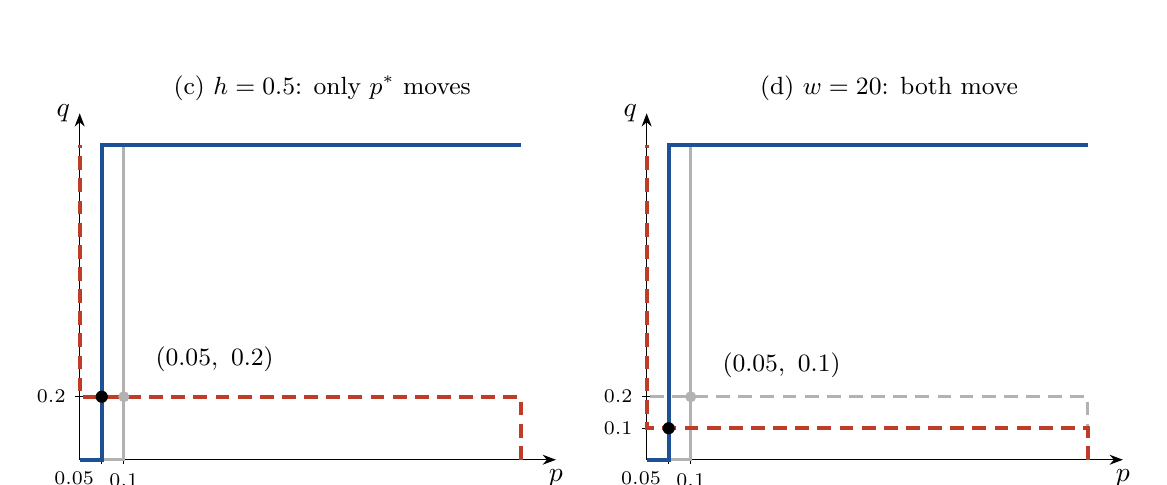
\begin{tikzpicture}[x=5.6cm,y=4.0cm,>=Stealth]
  \begin{scope}
    \draw[->] (0,0) -- (1.08,0) node[below] {$p$};
    \draw[->] (0,0) -- (0,1.1) node[left] {$q$};
    \draw (0.1,0.015) -- (0.1,-0.015) node[below] {\scriptsize $0.1$};
    \draw (0.05,0.015) -- (0.05,-0.015) node[below left=-1pt] {\scriptsize $0.05$};
    \draw (0.01,0.2) -- (-0.01,0.2) node[left] {\scriptsize $0.2$};
    \draw[gray!60,line width=1pt] (0,0) -- (0.1,0) -- (0.1,1) -- (1,1);
    \draw[mgr,line width=1.5pt] (0,0) -- (0.05,0) -- (0.05,1) -- (1,1);
    \draw[emp,line width=1.5pt,dash pattern=on 5pt off 3pt] (1,0) -- (1,0.2) -- (0,0.2) -- (0,1);
    \fill[gray!60] (0.1,0.2) circle (2pt);
    \fill (0.05,0.2) circle (2.2pt);
    \node[font=\small,anchor=west] at (0.15,0.32) {$(0.05,\ 0.2)$};
    \node[font=\small] at (0.55,1.18) {(c) $h = 0.5$: only $p^*$ moves};
  \end{scope}
  \begin{scope}[xshift=7.2cm]
    \draw[->] (0,0) -- (1.08,0) node[below] {$p$};
    \draw[->] (0,0) -- (0,1.1) node[left] {$q$};
    \draw (0.1,0.015) -- (0.1,-0.015) node[below] {\scriptsize $0.1$};
    \draw (0.05,0.015) -- (0.05,-0.015) node[below left=-1pt] {\scriptsize $0.05$};
    \draw (0.01,0.2) -- (-0.01,0.2) node[left] {\scriptsize $0.2$};
    \draw (0.01,0.1) -- (-0.01,0.1) node[left] {\scriptsize $0.1$};
    \draw[gray!60,line width=1pt] (0,0) -- (0.1,0) -- (0.1,1) -- (1,1);
    \draw[gray!60,line width=1pt,dash pattern=on 5pt off 3pt] (1,0) -- (1,0.2) -- (0,0.2);
    \draw[mgr,line width=1.5pt] (0,0) -- (0.05,0) -- (0.05,1) -- (1,1);
    \draw[emp,line width=1.5pt,dash pattern=on 5pt off 3pt] (1,0) -- (1,0.1) -- (0,0.1) -- (0,1);
    \fill[gray!60] (0.1,0.2) circle (2pt);
    \fill (0.05,0.1) circle (2.2pt);
    \node[font=\small,anchor=west] at (0.15,0.3) {$(0.05,\ 0.1)$};
    \node[font=\small] at (0.55,1.18) {(d) $w = 20$: both move};
  \end{scope}
\end{tikzpicture}
\caption{Comparative statics. Grey: the base case, equilibrium $(0.1, 0.2)$. Solid: manager's best
response; dashed: employee's. A change in the manager's payoffs ($h$) moves only the employee's
equilibrium mix, and vice versa; $w$ enters both players' payoffs.}
\label{fig:cs}
\end{figure}

\answer{Shirking halves ($p^* = 0.1 \to 0.05$) and so does monitoring ($q^* = 0.2 \to 0.1$). A
higher wage raises the employee's stake when caught (less monitoring keeps him indifferent) and the
manager's loss from an undetected shirker (less shirking keeps him indifferent). The employee gains
($8 \to 18$); the firm loses ($8 \to -1$): it buys the same drop in shirking as in (c) for $9$ more.}

%-------------------------------------------------------------------------------------------
\section*{(e) General formulas, policy, and the assumptions}

\subsection*{Equilibrium as a function of the parameters}

Repeating (b) with symbols, for $0 < g < w$ and $0 < h < w$:
\begin{align*}
  u_E(W, q) = u_E(S, q) &\iff w - g = (1 - q)\,w \iff q^* = \frac{g}{w},\\
  u_{M\!g}(M, p) = u_{M\!g}(N, p) &\iff (1 - p)(v - w) - h = (v - w) - p\,v \iff p\,w = h
  \iff p^* = \frac{h}{w}.
\end{align*}
Equilibrium payoffs:
\[
  u_E^* = w - g, \qquad
  \pi(w, h) := u_{M\!g}^* = (v - w) - p^* v = v - w - \frac{h v}{w}.
\]
\textbf{Comparative statics} (signs of the partial derivatives):
\begin{center}
\begin{tabular}{l|cccc}
 & $w$ & $g$ & $h$ & $v$ \\ \midrule
$p^* = h/w$ (shirking) & $-h/w^2 < 0$ & $0$ & $1/w > 0$ & $0$ \\
$q^* = g/w$ (monitoring) & $-g/w^2 < 0$ & $1/w > 0$ & $0$ & $0$
\end{tabular}
\end{center}
Shirking depends only on the manager's trade-off ($h$ against $w$); monitoring only on the employee's
($g$ against $w$). The value of output $v$ affects neither: it cancels from the manager's comparison
because monitoring does not change whether the work is done.

\textbf{The firm's payoff.} At the base values:
\[
  \frac{\partial \pi}{\partial h} = -\frac{v}{w} = -2, \qquad
  \frac{\partial \pi}{\partial w} = -1 + \frac{h v}{w^2} = -1 + \frac{20}{100} = -0.8, \qquad
  \frac{\partial \pi}{\partial v} = 1 - \frac{h}{w} = 0.9.
\]
A unit of wage costs the firm $1$ for sure and saves only $hv/w^2 = 0.2$ in output lost to shirking.
Inside the model, the wage that maximizes $\pi$ solves $\partial\pi/\partial w = 0$:
\[
  -1 + \frac{h v}{w^2} = 0 \ \Longrightarrow\ w^\dagger = \sqrt{h v} = \sqrt{20} \approx 4.47,
  \qquad \frac{\partial^2 \pi}{\partial w^2} = -\frac{2 h v}{w^3} < 0,
\]
with $\pi(w^\dagger) = v - 2\sqrt{hv} = 20 - 4\sqrt5 \approx 11.06$, $p^* \approx 0.224$ and
$q^* \approx 0.447$. Since $w^\dagger > g = 2$ and $w^\dagger > h = 1$, the game still has the mixed
equilibrium there. The employee would get only $w^\dagger - g \approx 2.47$: the model has no outside
option, so it ignores the \emph{participation constraint} $w - g \ge \bar u$. If the outside option
$\bar u$ exceeds $2.47$, the wage is set by participation, $w = g + \bar u$, not by incentives; at the
base wage the employee's 8 suggests that is the relevant case.

\subsection*{Policy recommendation}

\begin{enumerate}[label=\arabic*.]
  \item \textbf{Cheaper or better monitoring, not a higher wage.} Monitoring cost acts through
        $p^* = h/w$ and $\pi = v - w - hv/w$. Halving $h$ raises the firm's payoff from 8 to 9 and
        halves shirking; doubling the wage halves shirking just the same but drops the payoff to
        $-1$. With imperfect detection (a monitored shirker is caught with probability $\delta$), the
        same steps give
        \[
          p^* = \frac{h}{\delta w}, \qquad q^* = \frac{g}{\delta w}, \qquad
          \pi = v - w - \frac{h v}{\delta w},
        \]
        so what matters is the cost per detection, $h/\delta$: software that is cheaper ($h$ down) or
        more accurate ($\delta$ up) works the same way. Invest while the per-period cost of the
        upgrade is below the gain $v\,\Delta(h/\delta)/w$.
  \item \textbf{Do not try to ``monitor more''.} In equilibrium the monitoring rate is pinned at
        $g/w$ by the employee's indifference; a manager who simply monitors more is no longer best
        responding. The firm's levers are the parameters ($h$, $\delta$, $w$), or the timing.
  \item \textbf{Commit to an audit rate} (next subsection): announcing and hard-wiring random audits
        at rate $g/w = 20\%$ raises the payoff to $9.8$, and to $9.9$ combined with $h = 0.5$.
  \item \textbf{Keep the wage at the participation level.} The model says a raise is a poor
        anti-shirking tool in a one-shot relationship; whether the wage can be cut toward
        $\sqrt{hv}$ depends on the outside option, which the model omits.
\end{enumerate}
Ranking at the base values: commitment (9.8) $>$ cheaper monitoring (9) $>$ status quo (8) $>$
raising the wage to 20 ($-1$).

\subsection*{The commitment variant (Lecture 3 link)}

Change the timing: the manager \emph{first} announces, credibly, a monitoring probability $q$ (for
example, software that audits a random fraction $q$ of sessions); the employee observes $q$, then
chooses $W$ or $S$. Solve by backward induction (slides 29--30).

\emph{Employee (second mover).} He works iff $u_E(W, q) \ge u_E(S, q)$:
\[
  w - g \ge (1 - q)\, w \iff q \ge \frac{g}{w} = 0.2,
\]
breaking the tie toward $W$, as in a subgame-perfect equilibrium where the leader's payoff would
otherwise have no maximum.

\emph{Manager (first mover).} Any $q < g/w$ induces shirking and pays $q(-h) + (1 - q)(-w) < 0$. Any
$q \ge g/w$ induces work and pays $v - w - q h$, decreasing in $q$. So the manager commits to exactly
$q = g/w$:
\[
  p = 0, \qquad \pi^{\text{commit}} = v - w - \frac{h g}{w} = 20 - 10 - 1(0.2) = 9.8 > 8,
\]
a gain of $h(v - g)/w = 1.8$ over the simultaneous game. Even committing to monitor always (an
observable pure choice, to which the employee responds $W$) gives $v - w - h = 9 > 8$.

\emph{Why this is Lecture 3.} It is the Stackelberg logic of slide 37: a leader who can commit
picks the point on the follower's best response that suits him best. And it raises the
\emph{credibility} problem of sequential rationality (slides 29--30, 34; Tadelis \S8.3.4,
pp.~166--169, on time inconsistency): once the employee has worked, monitoring costs $h$ and catches
no one, so ex post the manager prefers $N$ (gain $h$, the first arrow in (a)). A promise to audit
that the manager can revise is not credible, and the employee, anticipating this, shirks. The
commitment must be hard-wired: an automated random audit, a contract with an outside auditor, or a
reputation built in a repeated relationship (Lectures 5--6).

\subsection*{Assumptions to question in the Itaú case}

\begin{itemize}
  \item \textbf{Perfect detection.} Activity software records keystrokes and mouse movement, not
        output; it misses some shirking ($\delta < 1$, which multiplies both $p^*$ and $q^*$ by
        $1/\delta$) and invites gaming (mouse jigglers).
  \item \textbf{Binary effort.} Real effort is continuous and multidimensional; an employee can
        ``work'' on what is measured and shirk on what is not. Monitoring inputs then distorts effort
        rather than raising it.
  \item \textbf{The penalty is only this period's wage.} At Itaú the penalty was dismissal, which
        also destroys the employee's future rents (seniority, a well-paid bank job relative to the
        outside option). If being caught costs $R \ge 0$ more, the employee's indifference becomes
        $w - g = (1 - q)\,w - q R$, so $q^* = g/(w + R)$: less monitoring is needed, and $p^* = h/w$
        is unchanged. This is the repeated game: the threat of losing a future rent is what makes
        \emph{efficiency wages} work (Lecture 6; Gibbons \S2.3.D, pp.~107--112; Milgrom and Roberts,
        pp.~250--255). It also qualifies (d): in a one-shot game a raise is a poor tool, but in a
        repeated one it raises the rent at stake.
  \item \textbf{No false positives; no legal constraints.} A worker flagged by mistake loses the
        wage although he worked, which lowers the return to working and calls for more monitoring
        to deter shirking. Processing employee activity data is subject to the LGPD (purpose,
        necessity, transparency) and dismissals for cause can be challenged in labour courts: both
        add to $h$ and cap how much monitoring is lawful.
  \item \textbf{Identical employees and one manager.} With heterogeneous effort costs $g$, some
        employees shirk at any audit rate and others never do; the firm would target monitoring on
        risk signals rather than audit at random. The population reading of $p^* = 10\%$ (slide 17)
        is only a stylized benchmark.
  \item \textbf{One-shot, simultaneous moves.} The relationship is repeated daily, employees learn
        whether software is installed, and audits can be conditioned on past records. Monitoring
        that is visible is closer to the commitment variant; continuous automated monitoring has a
        near-zero marginal $h$, which by $p^* = h/w$ drives shirking toward zero.
\end{itemize}

\answer{$p^* = h/w$ and $q^* = g/w$ (payoffs $w - g$ and $\pi = v - w - hv/w$). Recommend cheaper or
better monitoring (lower $h/\delta$): $\partial\pi/\partial h = -v/w = -2$, while a higher wage costs
more than it saves ($\partial\pi/\partial w = -0.8$; $w = 20$ gives $\pi = -1$), and in the model the
profit-maximizing wage is $\sqrt{hv} \approx 4.47$, if participation allows. Better still, commit to
a hard-wired random audit rate $g/w$: $p = 0$ and $\pi = 9.8$. Question: perfect detection, binary
effort, the wage as the only penalty (dismissal destroys future rents: repeated game, efficiency
wages), false positives and the LGPD, identical employees, and one-shot simultaneous timing.}

\end{document}
